\documentclass[12pt]{article}
\usepackage{hyperref}
\usepackage{amsmath, amssymb, amsfonts}
\usepackage[margin=1.2cm]{geometry}
\usepackage{xcolor}
\usepackage{graphicx}
\usepackage{enumitem}
\parindent 0pt
\newcommand{\lb}{\\$\left|\rightarrow\right.$}
\newcommand{\enter}{\\\textcolor{white}{1}}
\ExplSyntaxOn
\NewDocumentCommand{\bo}{m}
 {
   \bold_commas:n { #1 }
 }
\cs_new:Npn \bold_commas:n #1
 {
   \seq_set_split:Nnn \l_tmpa_seq { , } { #1 }
   \seq_map_indexed_function:NN \l_tmpa_seq \__bold_commas_aux:nn
 }
\cs_new:Npn \__bold_commas_aux:nn #1 #2
 {
   \textbf{#2}
   \int_compare:nNnTF { #1 } < { \seq_count:N \l_tmpa_seq }
     { , }
     { }
 }
\ExplSyntaxOff

\title{Artificial Intelligence (CT653 / CT710 / CT78506)\\[0.4em]\large Detailed PYQ, 2069--2082}
\author{}
\date{\today}

\begin{document}
\maketitle
\vspace{5cm}
\textbf{Notes}
\begin{itemize}[noitemsep]
  \item Questions from Tribhuvan University, IOE (2069--2082 BS), sorted by the CT710 syllabus. 41 papers.
  \item Regular exam = \bo{bold}, Back exam = regular font. A header printing ``Regular / Back'' in one box counts as Regular.
  \item The \textbf{course code} is a second, independent axis, and there are three of them:
  \begin{itemize}[noitemsep]
    \item \textbf{CT653}, BCT, III/II --- normal font. 26 papers, 2069--2082.
    \item \texttt{\textbf{CT710}}, BEI, IV/I --- \texttt{this monospace style}. 7 papers, 2079--2082.
    \item \textit{\textbf{CT78506}}, ``AI (Elective III)'', BEX, IV/II --- \textit{this italic style}. 8 papers, 2071--2077.
  \end{itemize}
  \item So: \bo{72 Ash} = CT653 Regular, 73 Ma = CT653 Back, \bo{\texttt{79 Bh}} = CT710 Regular, \texttt{81 Ba} = CT710 Back, \bo{\textit{77 Ch}} = CT78506 Regular, \textit{74 Ma} = CT78506 Back.
  \item \textbf{The same year code names different papers under different codes.} \bo{77 Ch} and \bo{\textit{77 Ch}} are two different papers, as are \bo{74 Bh}/\bo{\textit{74 Bh}}, \bo{73 Bh}/\bo{\textit{73 Bh}}, \bo{72 Ash}/\bo{\textit{72 Ash}}, 72 Ma/\textit{72 Ma} and \bo{71 Bh}/\bo{\textit{71 Bh}}. Only the font tells them apart --- 72 Ma and \textit{72 Ma} even print the same programme (BCT).
  \item Months: Ba = Baishakh, Jth = Jestha, Shr = Shrawan, Bh = Bhadra, Ash = Ashwin, Ka = Kartik, Po = Poush, Ma = Magh, Ch = Chaitra.
  \item Keywords: (I) = Importance/Need/Significance, (+) = Advantage, (-) = Disadvantage, +Fig = Figure/Diagram, +Eg = Example, Vs = Compare/Differentiate.
\end{itemize}
\pagebreak
\tableofcontents
\pagebreak

%=======================================================================
\section{Introduction}
\begin{center}(7 Hours)\end{center}

  \subsection{Definition of AI, Agents and the Turing Test}
    \begin{enumerate}[topsep=0pt, noitemsep]
      \item Define AI. When is a machine said to have passed the Turing test? Give two examples of constraint satisfaction problem. \hfill [2+5+1] (\bo{70 Bh})
        \lb What is AI? Explain the Turing test and its importance in AI. \hfill [7] (69 Po)
        \lb What is the importance of Turing Test in AI? List applications of AI. \hfill [2+4+2] (75 Ba)
        \lb Define AI. When is a machine said to have passed the Turing Test? Discuss two fields of application of AI. \hfill [2+3+3] (\bo{77 Ch})
        \lb List down disadvantages of AI. What is the importance of the Turing Test in Artificial Intelligence? What are the applications of AI? Explain. \hfill [2+2+4] (78 Ba)
        \lb What is knowledge and learning? Why are they important? Explain the factors that are required to pass the Turing test. \hfill [2+2+4] (79 Ash)
        \lb What is Turing test? How can it be used to measure intelligence of a machine? Explain. \hfill [2+5] (\bo{\texttt{79 Bh}})
        \lb Define intelligent agent. Explain the factors required to pass the Turing Test. \hfill [2+6] (\texttt{81 Ba})
        \lb What is Turing Test and total Turing test? Explain PEAS for a self-driving car. \hfill [4+4] (\bo{\textit{77 Ch}})
        \lb Describe Artificial Intelligence and its subfields. What is Total Turing Test? \hfill [4+3] (\bo{\textit{76 Bh}})

      \item If the Turing Test is passed, does this show that computers exhibit intelligence? State your reasons. \hfill [7] (72 Ma, \bo{73 Bh})
        \lb If the Turing test is passed, does this show that computer exhibit intelligence? Explain. Compare it with the Reverse Turing test with an example. \hfill [4+3] (\bo{\texttt{81 Bh}})
        \lb Can machine think? Explain your stance with appropriate reasons. Relate it with Turing Test and Reverse Turing Test. \hfill [2+4] (\bo{80 Ch})

      \item What is a rational agent? ``Systems that think like humans'' and ``systems that act like humans'' are part of AI --- justify with practical example. \hfill [1+6] (\bo{74 Bh})
        \lb Define AI and Intelligent agent. Differentiate between the different types of intelligent agent with examples. \hfill [2+6] (\bo{\texttt{80 Bh}})
        \lb What is Artificial Intelligence? Explain different types of Intelligent Agents with examples. \hfill [2+6] (80 Ash)
        \lb Define intelligent agent. Explain different types of intelligent agents and their interaction with environments alongwith appropriate examples. \hfill [1+6] (79 Jth)
        \lb What is an intelligent agent? How does a learning agent work? \hfill [8] (\bo{75 Bh})
        \lb Define AI. Justify that ``system that think rationally and act rationally'' is part of Artificial Intelligence. \hfill [8] (76 Ba)
        \lb What are the main growth areas of Artificial Intelligence? Describe with some implementations. Also compare and contrast between belief, hypothesis and knowledge. \hfill [4+4] (\bo{\textit{71 Bh}})

      \item PEAS --- describe the agent with its Performance measure, Environment, Actuators and Sensors.
        \lb What is an intelligent agent? What type of model does it work on? Explain PEAS for a Medical Diagnosis System. \hfill [2+2+3] (\texttt{80 Ba})
        \lb What are intelligent agents and how can we design an intelligent agent? Explain with examples with relevance to the PEAS framework. \hfill [4+4] (\bo{78 Ch}) [4+3] (\bo{\textit{74 Bh}})
        \lb What is an intelligent agent? Do we need PEAS for designing an intelligent agent? If so, define PEAS and provide the PEAS information for a Taxi Driver Agent and an Automated Robot in a manufacturing plant. \hfill [1+5] (81 Ash)
        \lb Define Artificial Intelligence. Design the PEAS information for an Automated Robot in a manufacturing plant. \hfill [2+3] (82 Ka)
        \lb What is intelligent agent? How can you design an intelligent agent? List down PEAS for a self-driving CAR. \hfill [2+6] (\texttt{82 Ba})
        \lb How can you define AI from the dimension of behavioral process and thought process? Using your own assumptions, design the PEAS framework for medicine delivery drones. \hfill [2+5] (\bo{\texttt{82 Bh}})

      \item Define AI. Differentiate between Natural (Human) Intelligence and Artificial Intelligence. Can AI replace humans? Justify. \hfill [1+3+4] (\bo{79 Ch})
        \lb Compare human intelligence and machine intelligence. Discuss some applications of Artificial Intelligence. \hfill [3+5] (78 Po)
        \lb What is Artificial Intelligence? What are the advantages and limitations of Artificial Intelligence over Natural Intelligence? \hfill [7] (\bo{\textit{73 Bh}})
    \end{enumerate}

  \subsection{Importance of AI}
    \begin{enumerate}[topsep=0pt, noitemsep]
      \item Growth areas, disadvantages and limitations of AI are asked inside the definition questions above --- see \bo{\textit{71 Bh}} (growth areas), 78 Ba (disadvantages) and \bo{\textit{73 Bh}} (limitations against natural intelligence).
    \end{enumerate}

  \subsection{AI and related fields}
    \begin{enumerate}[topsep=0pt, noitemsep]
      \item Describe Artificial Intelligence and its subfields. \hfill [4] (\bo{\textit{76 Bh}})
    \end{enumerate}

  \subsection{Brief history of AI}
    \begin{enumerate}[topsep=0pt, noitemsep]
      \item What is AI? Discuss brief history of AI with chronological development. \hfill [2+6] (70 Ma)
        \lb What is AI? Discuss history of AI in brief. \hfill [2+5] (\bo{71 Bh})
        \lb Define Artificial Intelligence stating the future prominence of the field. Which period was considered as the ``AI research failure'' period? Why? Write in brief. \hfill [7] (\textit{72 Ma})
    \end{enumerate}

  \subsection{Applications of AI}
    \begin{enumerate}[topsep=0pt, noitemsep]
      \item Discuss any two fields of your daily life where AI has been applied. \hfill [7] (\bo{69 Bh})
        \lb What is AI? Explain any two applications of AI in the real field. \hfill [7] (\bo{72 Ash})
        \lb Define AI. Describe the importance and practical application of AI. \hfill [6] (73 Ma)
        \lb How do you define Artificial Intelligence? Explain AI applications in different areas as a problem solving tool. \hfill [2+4] (\bo{81 Ch})
        \lb Also asked as the tail of a Turing-test question --- 75 Ba, \bo{77 Ch}, 78 Ba, 78 Po.
    \end{enumerate}

  \subsection{Definition and importance of Knowledge and Learning}
    \begin{enumerate}[topsep=0pt, noitemsep]
      \item Distinguish between knowledge and learning. What does acting humanly refer to? Explain. Define well defined problems. \hfill [2+5+1] (71 Ma)

      \item ``Learning is an essential characteristic for intelligent agents.'' Justify this statement. Write about the role of learning with a suitable example. \hfill [4+4] (\bo{73 Bh})
        \lb What is Artificial Intelligence, Knowledge and Learning? ``Learning is an essential characteristic for intelligent agents.'' Comment on this statement. \hfill [2+2+2+4] (\textit{74 Ma}, \bo{\textit{72 Ash}})
        \lb ``Learning is an essential characteristic for intelligent agents.'' Comment on this statement. Differentiate between Supervised and Unsupervised Learning. \hfill [4+4] (\bo{\textit{74 Bh}}, 79 Jth)

      \item Compare and contrast between belief, hypothesis and knowledge. \hfill [4] (\bo{\textit{71 Bh}})
    \end{enumerate}

\pagebreak
%=======================================================================
\section{Problem Solving}
\begin{center}(7 Hours)\end{center}

  \subsection{Defining problems as a state space search / Problem formulation}
    \begin{enumerate}[topsep=0pt, noitemsep]
      \item What are the steps of Problem solving? You are given three empty jugs: a 3-gallon, a 5-gallon and a 9-gallon, and a pump can fill water only in the 3-gallon jug. How do you get exactly 7 gallons in the 9-gallon jug? Formalize the problem, write production rules and draw the search tree. \hfill [2+1+2+3] (\bo{\texttt{79 Bh}})
        \lb Assume you are given two jugs, a 4-gallon one and a 3-gallon one, and a pump which has unlimited water. How can you get exactly 2 gallons of water in the 4-gallon jug? Formalize the problem, write down Production Rules and draw the Search Tree for the water jug problem. \hfill [2+2+4] (\bo{\textit{77 Ch}})
        \lb You are given two jugs, a 4-gallon one and a 3-gallon one. Neither has any measuring marker on it. There is a pump that can be used to fill the jugs with water. How can you get exactly 2 gallons of water into the 4-gallon jug? Solve it by specifying all steps and properties of problem solving. \hfill [4] (\bo{\textit{71 Bh}})
        \lb You are given two jugs, a 5-litre one and a 2-litre one. Neither has any measuring markers on it. There is a pump that can be used to fill the jugs with water. You are required to measure exactly 1 litre of water. Is this a well-defined problem? Justify your argument and list all the attributes to design an intelligent agent. Solve this problem by specifying states and the operations used. \hfill [8] (81 Ash)

      \item A farmer has a goat, a wolf and a cabbage on the west side of a river and wants to move everything to the east side. The boat holds the farmer and one other thing. The wolf eats the goat and the goat eats the cabbage if left alone. Formulate this puzzle as search and solve it (any method); draw the search tree and final solution. \hfill [8] (73 Ma)

      \item In problem solving, what is the concept of state space, state, successor function, goal test and path cost? \hfill [3] (\bo{\texttt{82 Bh}})
        \lb Discuss the steps involved in problem solving. \hfill [2] (\texttt{82 Ba})
        \lb What are the criteria for defining a problem? \hfill [2] (82 Ka)
        \lb Explain the steps of problem solving with a suitable example. \hfill [3] (\bo{81 Ch})
        \lb How do you define a problem in a state space? \hfill [3] (\bo{\textit{76 Bh}})
    \end{enumerate}

  \subsection{Well-defined problems}
    \begin{enumerate}[topsep=0pt, noitemsep]
      \item What makes a problem ``Well Defined''? Explain with a sample example of a state-space search framework. \hfill [3+4] (\bo{71 Bh})
        \lb What is problem space? (asked ahead of the crypto-arithmetic below). \hfill [2] (75 Ba)
        \lb Define the term well defined problem. \hfill [2] (80 Ash) [2] (\bo{78 Ch}) [2] (\texttt{81 Ba}) [2] (\bo{75 Bh})
        \lb List down the characteristics of a well-defined problem. \hfill [8] (81 Ash)
    \end{enumerate}

  \subsection{Constraint Satisfaction Problem (crypto-arithmetic)}
    \begin{enumerate}[topsep=0pt, noitemsep]
      \item Solve the following crypto-arithmetic problem through constraint satisfaction, showing all steps. Different letters denote different integers and identical letters denote the same integer.
        \lb LOGIC + LOGIC = PROLOG \hfill [7] (\bo{69 Bh}) [3+4] (72 Ma) [3+5] (\bo{79 Ch})
        \lb RIGHT + RIGHT = WRONG \hfill [7] (69 Po)
        \lb WRONG + WRONG = RIGHT \hfill [5+3] (\bo{70 Bh}) [2+6] (\bo{77 Ch})
        \lb ONE + ONE + TWO = FOUR \hfill [7] (71 Ma, \bo{73 Bh}) [2+6] (80 Ash)
        \lb TWO + TWO = FOUR \hfill [2+6] (\bo{78 Ch})
        \lb SEND + MORE = MONEY \hfill [1+6] (\bo{72 Ash}) [8] (76 Ba, \textit{74 Ma}, \bo{\textit{74 Bh}}, \bo{\textit{72 Ash}})
        \lb SWIM + WEAR = RELAX \hfill [1+6] (\bo{74 Bh}) [3+6] (\bo{81 Ch})
        \lb BASE + BALL = GAMES \hfill [2+6] (75 Ba, 82 Ka, \texttt{82 Ba}, 79 Ash) [3+5] (\bo{\texttt{82 Bh}}) [1+6] (79 Jth) [8] (\bo{\textit{73 Bh}})
        \lb TEN + TEN + FORTY = SIXTY \hfill [2+6] (\bo{\texttt{80 Bh}}, 78 Ba)
        \lb FORTY + TEN + TEN = SIXTY \hfill [2+6] (78 Po)
        \lb LOVE + LOVE = HATE \hfill [2+6] (\texttt{81 Ba})
        \lb EAT + THAT = APPLE \hfill [2+6] (\texttt{80 Ba}) [2+5] (\bo{80 Ch})
        \lb CROSS + ROADS = DANGER \hfill [2+6] (\bo{\texttt{81 Bh}})

      \item In a correctly worked out crypt-arithmetic problem AB + CD = AAA, what could be the possible values of B? Justify your answer. \hfill [4] (\bo{\textit{76 Bh}})

      \item What do you understand by Constraint Satisfaction Problem? Discuss it, and list all the constraints. \hfill [2] (\bo{\texttt{81 Bh}}, \bo{\texttt{80 Bh}}, \texttt{80 Ba}, 78 Ba, \bo{80 Ch}, \bo{\textit{74 Bh}}) [1] (79 Jth) [3] (\bo{79 Ch}) [2+6 asked as a whole] (\textit{74 Ma}, \bo{\textit{72 Ash}}, 78 Po)
        \lb Define AI. When is a machine said to have passed the Turing test? Give two examples of constraint satisfaction problem. \hfill [1] (\bo{70 Bh})
    \end{enumerate}

  \subsection{Game playing, Production systems}
    \begin{enumerate}[topsep=0pt, noitemsep]
      \item Why is searching necessary in AI? Explain the role of production system with a suitable example. \hfill [2+6] (70 Ma)
        \lb Define a production system. What are the essential terms or steps of a production system? \hfill [4] (\bo{\textit{71 Bh}}) [2] (82 Ka)
        \lb What do you understand by the Production system problem? \hfill [2] (\bo{77 Ch})
        \lb What do you understand about well defined problems? Explain about problems that can be solved using production rules with an example. \hfill [2+6] (\bo{75 Bh})

      \item Consider a Tic-Tac-Toe game playing as a problem. Prepare a brief description of your problem in terms of complete state-space, efficient data structures and goal, which are to be used for a machine to play that game. \hfill [7] (\textit{72 Ma})
    \end{enumerate}

\pagebreak
%=======================================================================
\section{Search Techniques}
\begin{center}(9 Hours)\end{center}

  \subsection{Necessity of searching and evaluation criteria}
    \begin{enumerate}[topsep=0pt, noitemsep]
      \item Explain the necessity of searching techniques in AI.
        \lb Searching is an important part of AI, justify it. Explain any two types of blind search and compare them in terms of space and time complexity. \hfill [2+7] (72 Ma)
        \lb Why is searching important in problem solving? What are the drawbacks of greedy best-first search and how does A* solve it? Explain with example. \hfill [2+7] (\bo{74 Bh}, \bo{78 Ch})
        \lb Why is searching important in problem solving? Differentiate between Depth first search and Breadth first search with their performance criteria. \hfill [2+6] (80 Ash)
        \lb What do you mean by Searching and what are the types of Search methods? \hfill [3] (82 Ka)

      \item On what basis can we evaluate the search algorithms? Explain. What are the approaches for Depth First Search and Depth Limit Search? Explain. \hfill [4+4] (79 Ash)
        \lb Discuss the evaluation criteria for a search algorithm. State the problems in the hill climbing search algorithm. \hfill [4+4] (\bo{75 Bh})
        \lb List down the approaches for evaluating searching methods. \hfill [2] (81 Ash)
    \end{enumerate}

  \subsection{Uninformed search --- DFS, BFS, depth limit search, comparison}
    \begin{enumerate}[topsep=0pt, noitemsep]
      \item What is a searching? Explain Breadth First Search and Depth First Search and compare their performance criteria. \hfill [9] (\bo{72 Ash})
        \lb What is blind search? Explain depth first search with an example and compare it with breadth first search. \hfill [9] (69 Po)
        \lb Differentiate between informed and blind search. How is depth first search different from breadth first search? Compare with evaluation parameters. \hfill [4+4] (\bo{70 Bh})
        \lb What is horn clause? Differentiate between Depth First Search and Breadth First Search. \hfill [1+7] (70 Ma)
        \lb Explain the necessity of searching techniques in AI. Differentiate between BFS and DFS with their performance criteria. \hfill [4+5] (\bo{73 Bh}) [7] (\bo{\texttt{79 Bh}})
        \lb Differentiate between depth first search and breadth first search with an example. \hfill [7] (79 Jth)
        \lb Compare breadth first search and depth first search along with examples. \hfill [8] (\bo{\textit{74 Bh}})
        \lb Describe Breadth First Search in detail. Also describe why Breadth First Search is Uninformed or blind search. \hfill [8] (\bo{\textit{71 Bh}})
        \lb Though BFS and DFS have some definite way of making search, they are still termed blind search --- why? Justify it, comparing with any one informed search technique. \hfill [7] (\textit{72 Ma})

      \item What is the advantage of depth limit search? Compare it with other search strategies. \hfill [4+4] (\bo{71 Bh})

      \item Make a detailed comparison between Informed and Uninformed search with examples. \hfill [8] (\textit{74 Ma})
        \lb Compare the informed and uninformed search techniques. What strategies can be employed to address the issue of local maxima in Hill Climbing Search? \hfill [4+4] (\texttt{81 Ba})
        \lb Compare informed and uninformed search. Explain how the Simulated Annealing algorithm overcomes the demerits of hill climbing search. \hfill [3+6] (\bo{\texttt{81 Bh}})
        \lb Explain about depth first and best first search and compare in terms of space and time complexity. \hfill [8] (\bo{\textit{72 Ash}})
    \end{enumerate}

  \subsection{Informed search --- hill climbing, best first, greedy, A*}
    \begin{enumerate}[topsep=0pt, noitemsep]
      \item Discuss the hill-climbing search algorithm along with the problems associated with it and their solutions. \hfill [9] (\bo{69 Bh})
        \lb Discuss the hill climbing search algorithm along with the problems associated with it and discuss their solutions. Why is simulated annealing important? \hfill [6+2] (75 Ba)
        \lb What are the problems associated with hill climbing search? Explain how simulated annealing overcomes them. \hfill [3+5] (\texttt{80 Ba})
        \lb State the problems in the hill climbing search algorithm. \hfill [4] (\bo{75 Bh})
        \lb Short note: Hill climbing problems / Hill climbing algorithm. \hfill [4] (\bo{77 Ch}) [4] (\bo{\texttt{79 Bh}})

      \item Devise an example to show how the A* algorithm uses path cost and heuristic cost to generate the best solution. \hfill [8] (73 Ma, \bo{\textit{77 Ch}})
        \lb Justify how the A* algorithm provides an optimum solution compared with the greedy search algorithm. \hfill [8] (78 Po)
        \lb Compare Greedy Search and A* search along with a simple example. \hfill [8] (\bo{\textit{73 Bh}})
        \lb What are the drawbacks of the greedy best first search method, and explain how the A* algorithm solves it with a suitable example. \hfill [2+6] (\texttt{82 Ba})
        \lb Explain A* search method using a suitable example. Discuss the drawbacks of the Hill Climbing Algorithm. \hfill [6+2] (78 Ba)
        \lb Define the terms admissibility and optimality in the context of A* search. Under what conditions is A* guaranteed to be both admissible and optimal? Provide justification for your answer. \hfill [4+5] (\bo{\texttt{82 Bh}})

      \item Explain the A* algorithm on the following figure, where the starting node is S and the destination is G. (Information in the node represents the cost required to reach the goal and information in the connecting link represents the cost from one node to the other.) \hfill [8] (\bo{81 Ch})\\
      \mbox{}\hfill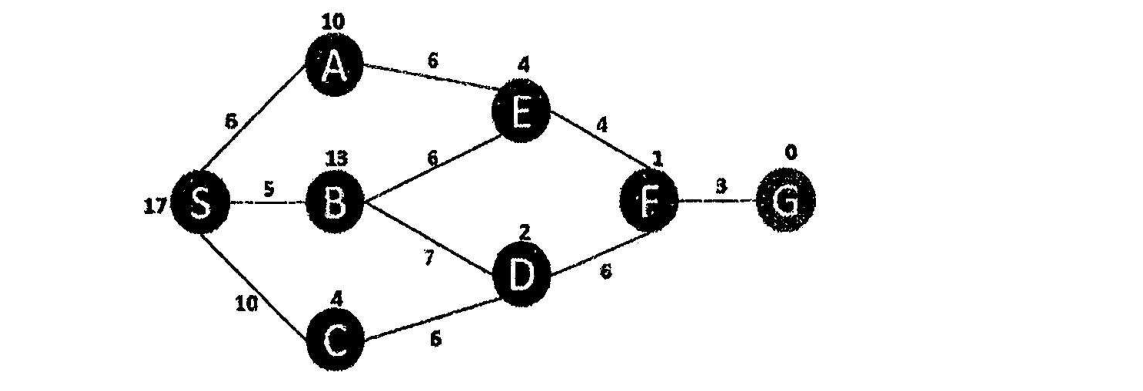
\includegraphics[width=4.6in]{images/ai_81ch_astar.png}\hfill\mbox{}

      \item How does A* search overcome the problem associated with Greedy Best First Search? Using the following figure and table, where the starting node is S and the destination is G, compare the result of the A* algorithm with greedy search. (The table gives the cost required to reach the goal; the connecting link gives the cost from one node to the other.) \hfill [3+4+3] (\bo{80 Ch})\\
      \mbox{}\hfill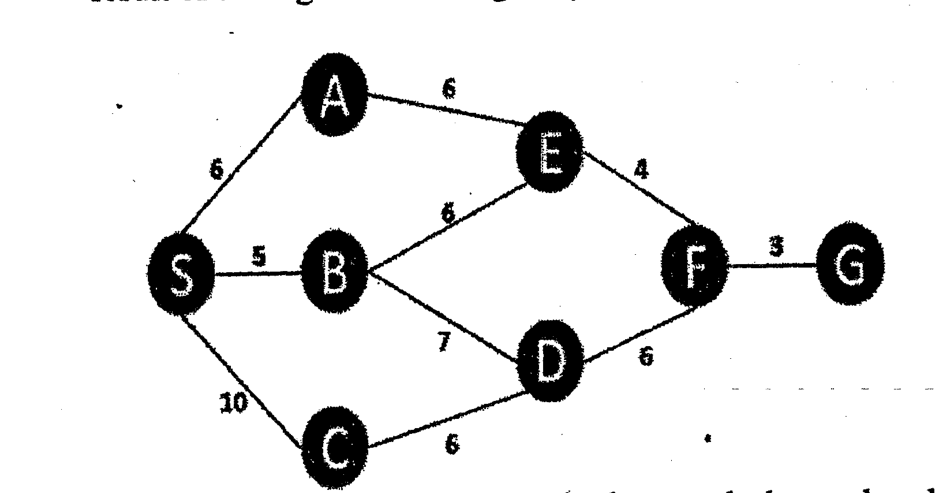
\includegraphics[width=3.9in]{images/ai_80ch_astar.png}\hfill\mbox{}
      \enter
      \begin{tabular}{|l|c|c|c|c|c|c|c|c|}
        \hline
        From & S & A & B & C & D & E & F & G \\ \hline
        Cost & 15 & 10 & 12 & 5 & 4 & 2 & 1 & 0 \\ \hline
      \end{tabular}

      \item Consider a search tree for a path-finding problem as shown. Assuming node A to be the root node and node I to be the goal node, explain how Best First Search reaches the goal by showing changes in the open list, closed list, and path at each step of the search. \hfill [5] (\bo{\textit{76 Bh}})\\
      \mbox{}\hfill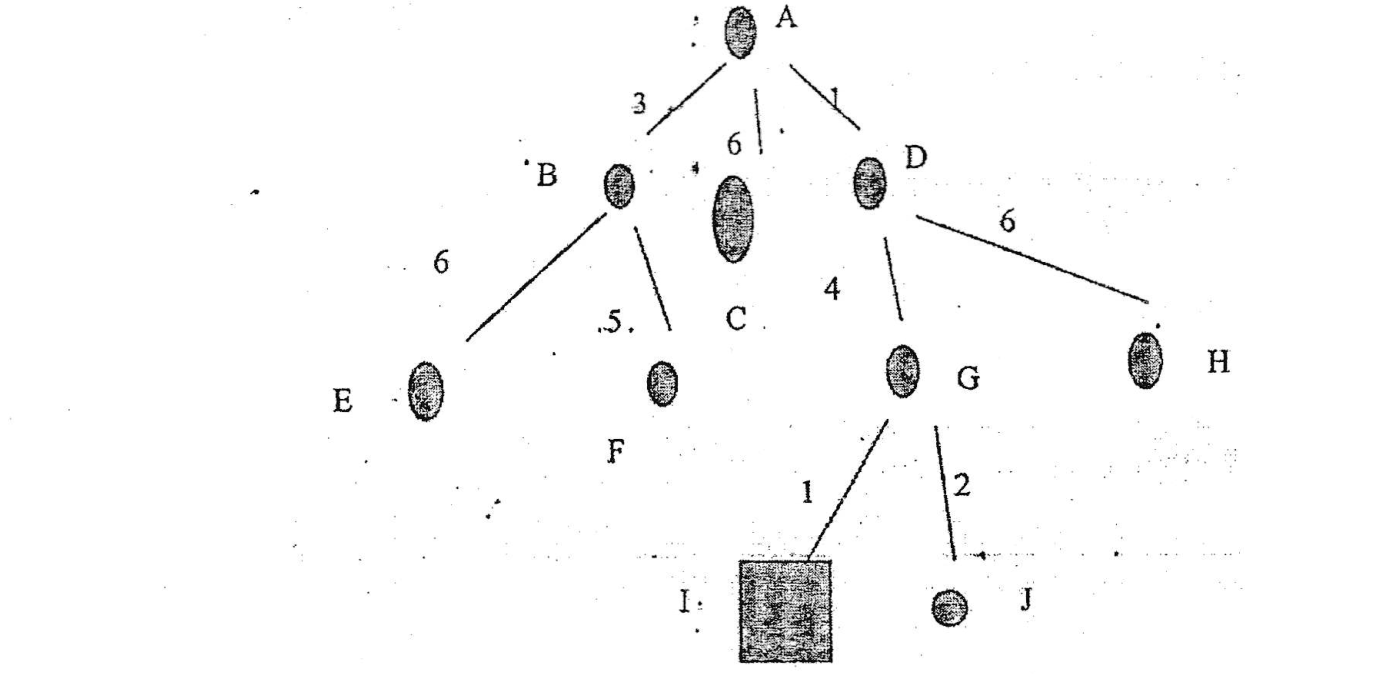
\includegraphics[width=4.6in]{images/ai_76bh_bfs.png}\hfill\mbox{}

      \item Short note: A* Search. \hfill [4] (\textit{72 Ma}, 79 Jth, \bo{\texttt{81 Bh}}) [3] (\texttt{80 Ba}, 76 Ba)
    \end{enumerate}

  \subsection{Adversarial search --- minimax, alpha-beta}
    \begin{enumerate}[topsep=0pt, noitemsep]
      \item How is informed search different from uninformed search? Explain the min-max algorithm with a suitable example, and discuss how alpha-beta is different from the min-max algorithm. \hfill [2+4+3] (71 Ma)
        \lb List out the disadvantages of the MIN-MAX algorithm for game playing and explain how Alpha-beta pruning helps to overcome the limitation of the MIN-MAX algorithm with an example. \hfill [2+6] (\bo{77 Ch})
        \lb What are the drawbacks of the Min-Max algorithm, and explain how the Alpha-Beta pruning algorithm solves it with a suitable example. \hfill [6] (82 Ka, 81 Ash)
        \lb Explain how alpha-beta pruning helps us reduce the complexity of adversarial search. \hfill [4] (\bo{\textit{76 Bh}})
        \lb How is searching done in adversarial search? How does A* search overcome the problem associated with Greedy Search? Explain with example. \hfill [2+6] (\bo{\texttt{80 Bh}})

      \item What is minmax search? Apply minmax search along with alpha-beta pruning for the following tree (max node at top). \hfill [2+6] (\bo{79 Ch})\\
      \mbox{}\hfill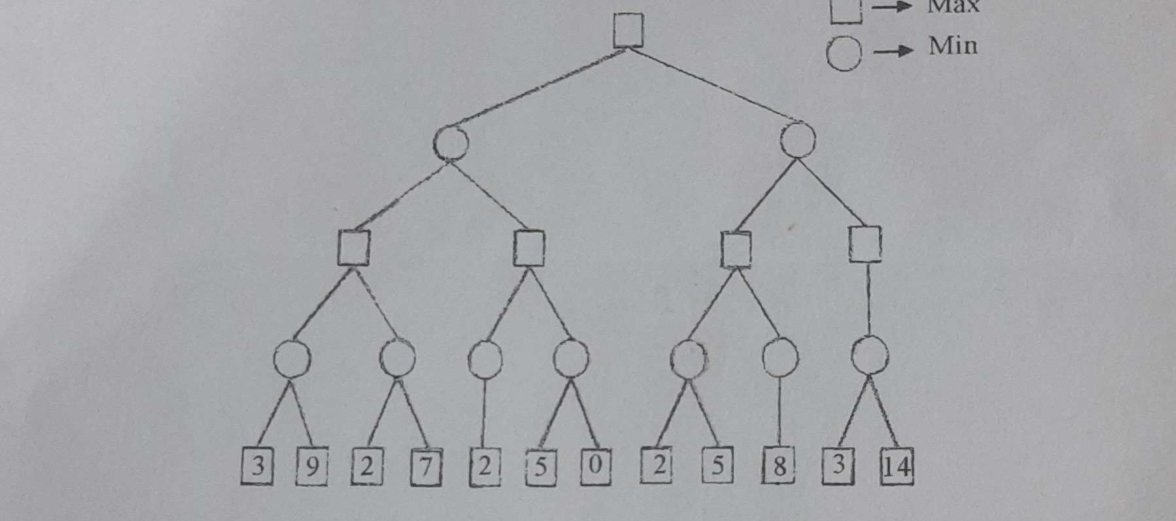
\includegraphics[width=4.8in]{images/ai_79ch_minmax.png}\hfill\mbox{}

      \item Discuss the alpha-beta pruning algorithm. Find the min-max value using this concept in the following tree. \hfill [4+4] (76 Ba)\\
      \mbox{}\hfill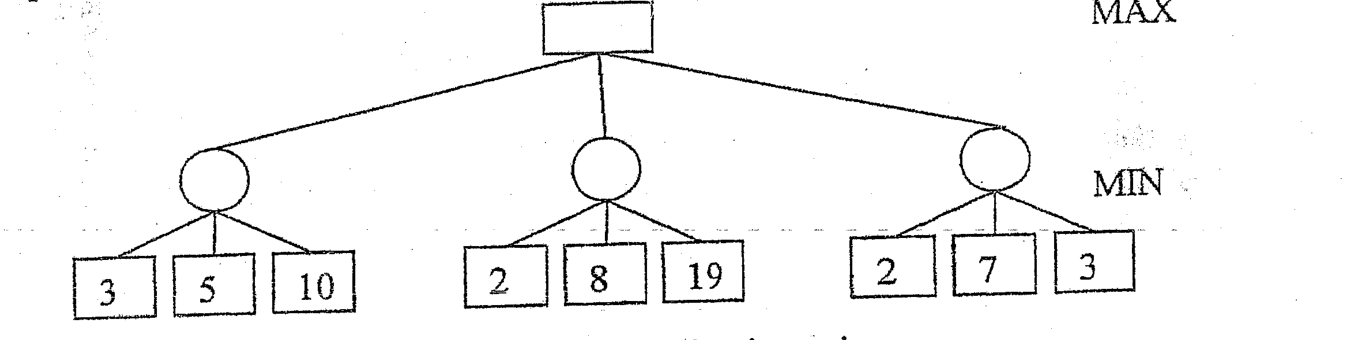
\includegraphics[width=4.6in]{images/ai_76ba_minmax.png}\hfill\mbox{}

      \item Short notes: Minmax algorithm; Alpha-beta pruning; Adversarial search. \hfill [4] (78 Ba, \bo{\textit{74 Bh}}, \textit{74 Ma}, \bo{\textit{72 Ash}}, 78 Po) [3] (\texttt{82 Ba})
    \end{enumerate}

\pagebreak
%=======================================================================
\section{Knowledge Representation, Inference and Reasoning}
\begin{center}(4 Hours)\end{center}

  \subsection{Formal logic, WFF and Conjunctive Normal Form (CNF)}
    \begin{enumerate}[topsep=0pt, noitemsep]
      \item Explain all the steps involved in conversion to conjunctive normal form (CNF) with a suitable example. \hfill [10] (69 Po) [8] (\bo{70 Bh})
        \lb Why is CNF required? Explain all the steps used to convert a quantified statement, with example. \hfill [2+6] (75 Ba)
        \lb Why is CNF necessary? Represent ``Everyone who loves all animals is loved by someone'' in FOPL and explain all the steps involved to convert it into CNF. \hfill [2+6] (\bo{79 Ch}, \bo{75 Bh})
        \lb What are the steps involved in converting FOL into CNF? \hfill [5] (\bo{\textit{76 Bh}})
        \lb List down the steps for converting to CNF and proof by resolution refutation. \hfill [3] (\bo{80 Ch})
        \lb What is CNF? Explain the rules of inference along with example. \hfill [2+3] (\bo{81 Ch})
        \lb Short note: Conjuctive Normal Form. \hfill [4] (76 Ba)

      \item Why is conjunctive normal form required? Explain all the steps to convert to CNF, and transform the given sentence(s) into CNF.
        \lb P $\vee$ ($\neg$P $\wedge$ Q $\wedge$ R); and ``Everyone who loves all animals is loved by someone.'' \hfill [2+2+2+3] (\bo{\textit{73 Bh}})
        \lb P $\rightarrow$ ((Q $\wedge$ $\neg$R) $\rightarrow$ S) \hfill [6] (\textit{74 Ma})
        \lb P $\rightarrow$ ((Q $\wedge$ $\neg$R) $\leftrightarrow$ S) \hfill [8] (\bo{\textit{72 Ash}})
        \lb (i) $\neg$(P $\wedge$ Q) $\vee$ (P $\vee$ S) $\rightarrow$ R \quad (ii) P $\rightarrow$ ((Q $\wedge$ $\neg$R) $\leftrightarrow$ S) \hfill [2+2+4] (79 Jth)

      \item Define a WFF with its properties. Prove that the proposition (A $\wedge$ (A $\rightarrow$ B) $\rightarrow$ B) is a tautology. \hfill [4+4] (\bo{\textit{71 Bh}})
    \end{enumerate}

  \subsection{Propositional / predicate logic, FOPL, Horn clauses, Skolemization}
    \begin{enumerate}[topsep=0pt, noitemsep]
      \item Why do we need FOPL? State any three rules of inference. How can we make a machine with learning capacity? \hfill [2+3+3] (70 Ma)
        \lb List the rules of inference. When can we use these rules? Explain. \hfill [3] (\bo{78 Ch}) [3] (80 Ash)

      \item Define skolemization with example. \hfill [2] (\texttt{81 Ba}) \quad (also a short note, \bo{69 Bh})

      \item Define horn clause with example. \hfill [3] (\bo{78 Ch}) \quad (also asked with DFS/BFS, 70 Ma)

      \item Convert the following into FOL. \hfill [2] (\bo{\textit{76 Bh}})
        \lb a) Arya hates Joffery and Cersei. b) No Lannister loves Bran. c) Sansa has at least one sister. d) Every Stark hates at least one Lannister.

      \item Short note: Predicate logic; Sentence validity. \hfill [4] (\bo{75 Bh}, \textit{72 Ma})
    \end{enumerate}

  \subsection{Rules of inference, unification, resolution refutation, deduction}
    \begin{enumerate}[topsep=0pt, noitemsep]
      \item Prove the goal using FOPL / resolution refutation from the given premises:
        \lb Every American who sells weapons to hostile nations is a criminal. The country Abc is enemy of America. All of the missiles in Abc were sold by John. John is an American. Prove John is a criminal. \hfill [10] (\bo{69 Bh})
        \lb Every American who sells weapons to hostile nations is a criminal. The country XYZ is enemy of America. All of its missiles in XYZ were sold by Donald, who is an American. Prove that Donald is a criminal using FOPL based resolution refutation. \hfill [8] (75 Ba)
        \lb It is a crime for an American to sell weapons to hostile nations. Nono has some missiles. All the missiles owned by Nono were sold to it by Colonel West. Missiles are weapons. An enemy of America counts as hostile. Colonel West is an American. The country Nono is an enemy of America. Prove that Colonel West is a criminal by using FOPL based Resolution Refutation. \hfill [8] (\bo{77 Ch}, 82 Ka)
        \lb The law says that it is a crime for an American to sell weapons to hostile nations. The country Nono, an enemy of America, has some missiles, and all of its missiles were sold to it by Colonel West, who is American. Prove that Col. West is criminal using \textbf{forward chaining}. \hfill [2+6] (81 Ash)
        \lb Every American who sells weapons to hostile nations is a criminal. Every enemy of America is a hostile. Nono has some missiles. All missiles of Nono were sold by Gorge. Gorge is an American. Nono is a Country. Nono is the enemy of America. Missiles are weapons. Prove that ``Is Gorge a criminal?'' using Resolution by Refutation. \hfill [9] (\bo{\texttt{81 Bh}})
        \lb It is a crime for a Nepali to sell weapons to an enemy of Nepal. Mr.\ A is an enemy of Nepal. Mr.\ A has some missiles. Missiles are weapons. Mr.\ R is a Nepali. If Mr.\ A has missiles then those missiles were sold to Mr.\ A by Mr.\ R. Prove ``Mr.\ A is a criminal''. \hfill [6] (\bo{\texttt{82 Bh}})
        \lb All oversmart persons are stupid. Children of oversmart persons are naughty. Ram is children of Hari. Hari is oversmart. Show that Ram is naughty using FOPL based resolution. \hfill [8] (\bo{70 Bh})
        \lb If X is on the top of Y, Y supports X. If X is above Y and they are touching each other, X is on the top of Y. A cup is above a book. A cup is touching a book. Show that supports(book, cup) is true. \hfill [8] (\bo{71 Bh})
        \lb Assume the following facts: John likes all kinds of food; apples are food; chicken is food; anything anyone eats and isn't killed by is food; Bill eats peanuts and is still alive; Sue eats everything Bill eats. Prove that John likes peanuts using resolution refutation. \hfill [7] (\bo{72 Ash}) [8] (\bo{74 Bh}, \bo{\textit{73 Bh}})
        \lb Assume the following facts: a) Ram likes all kinds of food; b) Apples are food; c) Chicken is food; d) Anything anyone eats and is not killed by is food; e) Krishna eats peanuts and is still alive; f) Radha eats everything Krishna eats. Prove the statement ``Ram likes peanut'' using resolution. \hfill [8] (\bo{\textit{71 Bh}})
        \lb Assume the following facts: i) Ram likes all kinds of food; ii) apples and vegetables are food; iii) anything anyone eats and not killed is food; iv) Anil eats peanuts and is still alive; v) Ram eats everything that Anil eats. Prove that ``Ram likes peanuts'' using resolution refutation. \hfill [8] (\bo{\texttt{80 Bh}})
        \lb Assume the following facts: a) Sita likes all kinds of food; b) Momo and Burger are food; c) anything anyone eats and isn't killed by is food; d) Bill eats mushroom and is still alive; e) Sue eats everything Bill eats. Prove that ``Sita likes mushroom'' using resolution refutation method. \hfill [8] (\texttt{80 Ba})
        \lb Bhogendra likes all kinds of food. Oranges are food. Chicken is food. Anything anyone eats and isn't killed by is food. If a person likes a food it means that person has eaten it. Jogendra eats peanuts and is still alive. Shailendri eats everything Bhogendra eats. Express them in FOPL, put them into clause form, and use resolution to prove that Shailendri likes chicken. \hfill [6+4] (\textit{72 Ma})
        \lb Using resolution, solve the following statements: All pompeian are Romans. All Romans were either loyal to Caesor or hated him. Everyone is loyal to someone. People only try to assassinate rulers they not loyal to. Marcus tried to assassinate Caesor. Marcus was pompeian. Find, did Marcus Caesor? \hfill [7] (72 Ma)
        \lb Assume the following facts: i) horses, cows, pigs are mammals; ii) an offspring of a horse is a horse; iii) Bluebeard is a horse; iv) Bluebeard is Charlie's parent; v) offspring and parent are inverse relations; vi) every mammal has a parent. Prove Charlie is a horse using resolution refutation. \hfill [8] (\bo{73 Bh}, 78 Po, \bo{\textit{74 Bh}}) [6] (79 Jth)
        \lb Prove that ``Charlie is a mammal'' with given propositions: a) cows, pigs and horses are mammal; b) the child of horse is a horse; c) Bluebeard is a horse; d) Bluebeard is Charlie's father; e) child and father are inverse relation; f) every mammal has a father. \hfill [8] (\bo{\texttt{79 Bh}})
        \lb Assume the following facts: (i) Cow, Buffalo, Bull are mammals; (ii) an offspring of a Cow is Cow; (iii) Kali is a Cow; (iv) Kali is Taarey's parent; (v) offspring and parent are inverse relations; (vi) every mammal has a parent. By using resolution refutation, prove that Taarey is a Cow. \hfill [8] (78 Ba)
        \lb Consider the following axioms: i) anyone whom Mary loves is a football star; ii) any student who does not pass does not play; iii) John is a student; iv) any student who does not study does not pass; v) anyone who does not play is not a football star. Prove that ``If John does not study, then Mary does not love John'' using resolution by refutation. \hfill [10] (73 Ma)
        \lb Define skolemization with example. Consider the following axioms: a) anyone passing his engineering exams and winning the lottery is happy; b) anyone who studies or is lucky can pass all his exams; c) Sneha did not study but she is lucky; d) anyone who is lucky wins the lottery. Using resolution refutation, prove that Sneha is happy. \hfill [2+6] (\texttt{81 Ba})
        \lb Every child loves Santa. Everyone who loves Santa loves any reindeer. Rudolph is a reindeer, and Rudolph has a red nose. Anything which has a red nose is weird or is a clown. No reindeer is a clown. Scrooge does not love anything which is weird. Using Resolution Refutation, derive the conclusion: Scrooge is not a child. \hfill [8] (\bo{81 Ch})
        \lb Define horn clause with example. Consider the same six Santa / Rudolph / Scrooge axioms. Represent these axioms in predicate calculus and then convert each formula to CNF. List down the rules of inference. When can we use these rules? Explain. \hfill [3+3] (\bo{78 Ch})
        \lb Convert the following sentences into FOPL and answer ``Did Curiosity kill the cat'' by resolution refutation: a) Everyone who loves all animals is loved by someone. b) Anyone who kills an animal is loved by no one. c) Jack loves all animals. d) Either Jack or Curiosity killed the cat. \hfill [3+5] (\bo{80 Ch})
        \lb List the rules of inference. Convert the following into FOPL and prove using Resolution Refutation System: ``All people who are not poor and are smart are happy. Those people who can read are not stupid. John can read and is wealthy. Happy people have exciting lives. Can anyone be found with an exciting life?'' \hfill [3+5] (80 Ash)
        \lb Assume the following facts: a) Steve only likes easy courses; b) Science courses are hard; c) All the courses in the basket weaving department are easy; d) BK301 is a basket weaving course. Prove that Steve likes BK301 using Resolution Refutation. \hfill [7] (79 Ash)
        \lb List down the rule for Inference. Consider the following axioms: All hounds howl at night. Anyone who has any cats will not have any mice. Light sleepers do not have anything which howls at night. John has either a cat or a hound. Prove: ``If John is a light sleeper, then John does not have any mice'' by resolution refutation. \hfill [2+8] (76 Ba)
        \lb Consider the following axioms: All direwolves howl at night. Anyone who has any cat will not have any mice. Light sleepers do not have anything that howls at night. Jon has either a cat or a direwolf. Prove that if Jon is a light sleeper, then Jon does not have any mice, using the resolution method. \hfill [7] (\bo{\textit{76 Bh}})
        \lb If it is a sunny and warm day you will enjoy. If it is a warm and pleasant day you will do strawberry picking. If it is raining, no strawberry picking. If it is raining you will get wet. It is a warm day. It is raining. It is sunny. Prove that ``You will enjoy'' using resolution by refutation. \hfill [8] (\bo{\textit{77 Ch}})

      \item What is rule based reasoning? Explain Backward Chaining with a suitable example. \hfill [7] (72 Ma)
        \lb Explain backward chaining with a suitable example and compare with forward chaining. \hfill [4+4] (70 Ma)
        \lb Explain Backward Chaining with a suitable example. \hfill [7] (\bo{71 Bh})
        \lb What is rule-based reasoning? Explain with an example. \hfill [2] (\bo{77 Ch})

      \item What is knowledge, representation and reasoning? Describe forward chaining with a practical example. \hfill [2+5] (\bo{72 Ash})
        \lb Explain forward chaining giving a suitable example. \hfill [8] (78 Po, \bo{\textit{77 Ch}})
        \lb Differentiate between forward and backward chaining using a suitable example. \hfill [4] (\bo{74 Bh}) [7] (\bo{\texttt{79 Bh}}, \bo{\texttt{81 Bh}}) [2+4] (82 Ka) [2] (81 Ash) [3] (\bo{\textit{73 Bh}}) [4] (\bo{80 Ch}, short note)

      \item What is a knowledge-based agent? How does it work? Explain with examples. \hfill [2+3+2] (\texttt{82 Ba})
    \end{enumerate}

  \subsection{Statistical reasoning --- Probability, Bayes' theorem, causal/belief networks}
    \begin{enumerate}[topsep=0pt, noitemsep]
      \item What is causal network? Explain reasoning in belief network with suitable example. \hfill [2+5] (71 Ma)
        \lb What is belief network? How reasoning is done in this network? \hfill [2+6] (\bo{79 Ch})
        \lb Why is probabilistic reasoning important in AI? When do we use a Bayesian Network? Explain. \hfill [3+6] (79 Ash)
        \lb What are the approaches for measuring uncertainty? \hfill [2] (81 Ash)
        \lb How is reasoning done under uncertainty? \hfill [3] (80 Ash)
        \lb Explain how statistical reasoning aids inference and reasoning in the light of Bayes' theorem. \hfill [3] (\bo{78 Ch})
        \lb How is Bayes' theorem used in a belief network? \hfill [6] (\bo{77 Ch})

      \item What is causal net? How does Bayes' Theorem calculate the probability in a causal net? Explain with example calculation. \hfill [7] (\bo{73 Bh})
        \lb What is neural network? Describe its types. A doctor knows that the disease meningitis causes the patient to have a stiff neck 50\% of the time. The doctor also knows that the probability that a patient has meningitis is 1/50,000, and the probability that any patient has a stiff neck is 1/20. Find the probability that a patient with a stiff neck has meningitis? \hfill [3+5] (71 Ma)
        \lb What is prior probability and posterior probability? A doctor knows that the disease meningitis causes a patient to have a stiff neck, say, 80\% of the time. The doctor also knows some unconditional facts: the prior probability that any patient has meningitis is 1/50000, and the prior probability that any patient has a stiff neck is 1\%. Determine the probability of meningitis when a patient has a stiff neck. \hfill [2+6] (\texttt{81 Ba})
        \lb A doctor is called to see a sick child. The doctor has prior information that 90\% of sick children in that neighborhood have the flu, while the other 10\% are sick with measles. Let F stand for an event of a child being sick with Flu and M stand for an event of a child being sick with measles. Assume for simplicity that there no other maladies in that neighborhood. A well-known (and common) symptom of measles is a rash and has probability of 0.95. However, very occasionally, children with flu also develop rash and has probability of 0.08. Upon examining the child, the doctor finds a rash. What is the probability that the child has measles? \hfill [8] (73 Ma)
        \lb What is Prior Probability and Posterior Probability, and show how these probabilities are used in Bayes' Theorem. Is there any connection between Belief Network and Bayes' Theorem? Justify with an example. \hfill [3+5] (\bo{80 Ch})

      \item What do you understand by Bayesian Network? In a County, 51\% of the adults are males and the other 49\% are females. One adult is randomly selected for a survey involving credit card usage. i) Find the prior probability that the selected person is a male. ii) It is later learned that the selected survey subject was smoking a cigar. Also, 9.5\% of males smoke cigars, whereas 1.7\% of females smoke cigars (based on data from the Substance Abuse and Mental Health Services Administration). Use this additional information to find the probability that the selected subject is a male. \hfill [2+6] (\bo{\texttt{80 Bh}}) [8] (\bo{\textit{73 Bh}})
        \lb What is Bayesian network? Describe with an appropriate example. How inference can be done using this network? \hfill [5+3] (\texttt{80 Ba})

      \item After your yearly checkup, the doctor has bad news and good news. The bad news is that you tested positive for a serious disease, and that the test is 99\% accurate (i.e.\ the probability of testing positive given that you have the disease is 0.99, as is the probability of testing negative given that you don't have the disease). The good news is that this is a rare disease, striking only one in 10,000 people. Why is it good news that the disease is rare? What are the chances that you actually have the disease? \hfill [8] (\bo{\textit{72 Ash}})

      \item What are the approaches for measuring uncertainty? 1\% of people have a certain genetic defect. 90\% of tests for the gene detect the defect (true positives). 10\% of the tests are false positives. a) What might be the probability of getting the genetic defect result? b) If a person gets a positive test result, what are the odds they actually don't have the genetic defect? \hfill [2+6] (81 Ash)

      \item How is reasoning done under uncertainty? Three factories produce light bulbs to supply the market. Factory A produces 20\%, 50\% of the bulbs are produced in factory B and 30\% in factory C. 2\% of the bulbs produced in factory A, 5\% of the bulbs produced in factory B and 3\% of the bulbs produced in factory C are defective. A bulb is selected at random in the market and found to be defective. What is the probability that this bulb was produced by factory B? \hfill [3+5] (80 Ash)

      \item Explain how statistical reasoning aids in inference and reasoning in light of Bayes' theorem. At a certain University, 5\% of men are over 6 feet tall and 2\% of women are 6 feet tall. 60\% of students are female. If a student is selected at random from among all those over six feet tall, what is the probability that the selected student is a woman? \hfill [3+5] (\bo{78 Ch})

      \item What are casual networks? Given the following statistics, what is the probability that a woman has cancer if she has a positive mammogram result? i) One percent of women over 50 have breast cancer. ii) Ninety percent of women who have breast cancer test positive on mammograms. iii) Eight percent of women will have false positives. \hfill [2+6] (\texttt{82 Ba})

      \item A Bayesian Belief Network (BBN) is used in a medical diagnosis system. The network includes the binary variables C (Patient has Cancer), T (Test result is Positive) and S (Patient is a Smoker), with structure S $\rightarrow$ C $\rightarrow$ T and conditional probabilities P(S=Yes)=0.3, P(C=Yes\,$|$\,S=Yes)=0.2, P(C=Yes\,$|$\,S=No)=0.05, P(T=Yes\,$|$\,C=Yes)=0.9, P(T=Yes\,$|$\,C=No)=0.1. Explain how the Bayesian Belief Network enables reasoning under uncertainty in this medical context. \hfill [7] (\bo{\texttt{82 Bh}})

      \item What do you understand by Bayesian Network? For the given Bayesian network below, find the probability of grass being wet when the weather is cloudy, there is some sprinkler but no rain, i.e.\ C = True, S = True, R = False and W = True. \hfill [2+6] (78 Ba)\\
      \mbox{}\hfill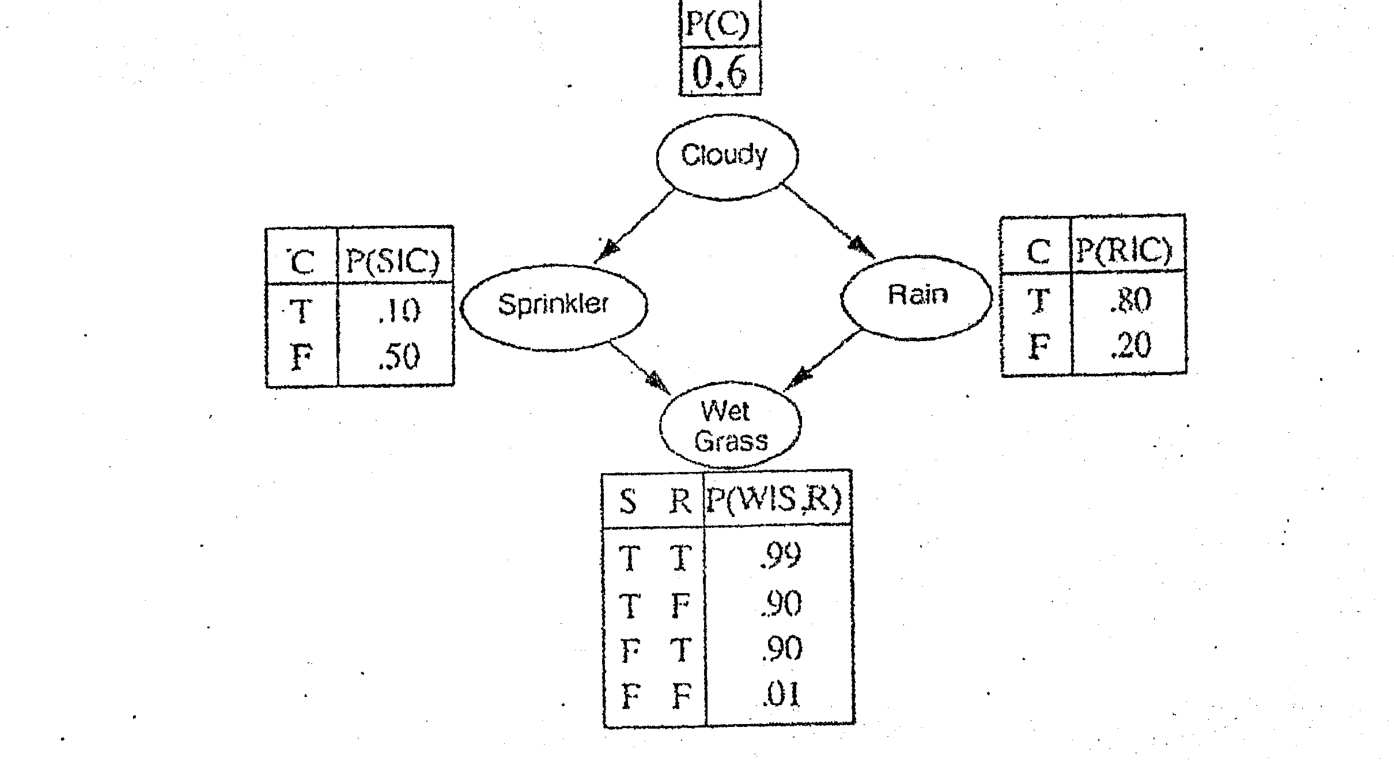
\includegraphics[width=4.2in]{images/ai_78ba_bbn.png}\hfill\mbox{}
    \end{enumerate}

\pagebreak
%=======================================================================
\section{Structured Knowledge Representation}
\begin{center}(4 Hours)\end{center}

  \subsection{Approaches and Issues in Knowledge Representation}
    \begin{enumerate}[topsep=0pt, noitemsep]
      \item What are the different knowledge representation models? Discuss semantic nets with an example. \hfill [7] (\bo{69 Bh}) [2+5] (\texttt{80 Ba})
        \lb Explain in detail four types of Knowledge Representation Scheme. \hfill [8] (\bo{\textit{73 Bh}})
        \lb What are the different approaches for knowledge representation? List down the essential properties and issues of the knowledge representation system. \hfill [4+2+2] (79 Ash)
        \lb Explain the different approaches of knowledge representation. Highlight the pros and cons of Semantic Nets and Frames. \hfill [2] (\bo{\texttt{81 Bh}})
        \lb What do you understand by structured knowledge representation? Explain semantic nets. \hfill [2+5] (\bo{\textit{76 Bh}})

      \item How is a knowledge representation evaluated? Explain semantic net and frame representation with examples. \hfill [3+5] (\bo{\texttt{80 Bh}})
        \lb Discuss the different approaches to knowledge representation. How do you make a choice among these approaches? Is it possible to evaluate the knowledge representation? List down any issues associated with it. \hfill [2+2+2+2] (\bo{80 Ch})
        \lb What are the different issues in knowledge representation? Discuss the importance of frame in knowledge representation with a suitable example. \hfill [3+5] (80 Ash)
        \lb What are the different issues in knowledge representation? \hfill [2] (\bo{\texttt{82 Bh}}) [2] (\bo{\textit{76 Bh}}, in an expert system)
        \lb List the issues need to be consider in Knowledge Representation techniques. Convert the given sentences into a Semantic Network (sentence list under \textit{Semantic nets} below). \hfill [2+6] (\bo{\texttt{79 Bh}})
        \lb What is knowledge representation? How is a semantic network used to represent knowledge? \hfill [2+6] (\bo{75 Bh})
    \end{enumerate}

  \subsection{Semantic nets}
    \begin{enumerate}[topsep=0pt, noitemsep]
      \item What is semantic net? Explain with a suitable example. \hfill [8] (\bo{70 Bh})
        \lb What is a semantic net? Draw a sample net about your course AI to demonstrate the knowledge representation features and qualities of a semantic net. \hfill [7] (\textit{72 Ma})
        \lb When do we use a semantic network? \hfill [2] (\texttt{82 Ba})

      \item Convert the given sentences into a Semantic Network.
        \lb i) A person is a mammal. ii) Sakti Gauchan is a person. iii) Person has nose. iv) Sakti Gauchan is in Nepalese team. v) Uniform color of Sakti Gauchan is Red/Blue. \hfill [7] (72 Ma)
        \lb A person is a mammal. Sandeep Lamichane is a person. Person has nose. Sandeep Lamichane is in the Nepalese cricket team. Uniform color of Sakti Gauchan is Red/Blue. \hfill [2+6] (78 Po)
        \lb i) The height of the adult male is 5.10. ii) Baseball player is an adult male. iii) Adult male is a person. iv) Batting average of Baseball players is 0.252. v) Pee-wee-Reese is a Fielder. vi) Fielder is Baseball player. vii) Team of Pee-wee-Reese is Brooklyn Dodger. \hfill [7] (\bo{73 Bh})
        \lb i) The avg height of an adult is 5'6''. ii) Cricket player is an adult male. iii) Adult male is a person. iv) Batting average of a cricket player is 37.59. v) Rohit Paudel is a Fielder. vi) Fielder is a cricket player. vii) Team of Rohit Paudel is Nepal. \hfill [2+6] (\bo{79 Ch})
        \lb a) Tom is a cat. b) Tom fights with rat. c) Tom is owned by Ram. d) Tom is black in color. e) Cats like milk. f) Rats like cheese. g) The cat sat on the bed. h) A cat is a mammal. i) A Rat is an animal. j) All mammals are animals. k) Every mammal gives birth a baby. \hfill [2+6] (\bo{\texttt{79 Bh}})
        \lb Tom is a cat. Tom caught a bird. Tom is owned by Sudeep. Tom is ginger in color. Cats like cream. The cat sat on the mat. A cat is a mammal. A bird is an animal. All mammals are animals. Mammals have fur. Sudeep age is 20. \hfill [2+5] (\bo{\texttt{82 Bh}}) [2+6] (\bo{81 Ch})
        \lb Cat is a mammal. Cat has fur. Mammal has vertebra. Mammal is an animal. Bear is a mammal. Bear has fur. Whale is a mammal. Whale lives in water. Fish is an animal 10. Fish lives in water. \hfill [1+6] (82 Ka)
        \lb Figo is a dog. Fido is own by Rohit. Fido is ginger in color. Dog is a mammal. All Mammals are animals. Mammals have fur. \hfill [2+6] (\bo{\texttt{81 Bh}})
        \lb i) Employee is a human. ii) Hari is an employee. iii) Sita is a human. iv) Supervisor is a human. v) Ram is a supervisor. vi) Ram is married to Sita. vii) Ram is supervisor of Hari. \hfill [2+6] (\texttt{82 Ba})
        \lb Convert into FOPL and represent using a semantic network: i) Ram is a person. ii) Person is an animal. iii) Ram likes Jhilke. iv) Jhilke is a cat. v) Cat eats fish. vi) Cat is an animal. vii) fish is an animal. \hfill [2+6] (81 Ash)
        \lb Tweety and Sweety are birds. Tweety has a red beak. Sweety is Tweety's child. A crow is a bird. Birds can fly. Sparrow is a bird. Sparrow has a wing. \hfill [2+6] (\bo{\textit{77 Ch}})

      \item Give an example of learning by analogy. How can knowledge be represented using a semantic network? Explain with example. \hfill [1+7] (\bo{71 Bh})
    \end{enumerate}

  \subsection{Frames}
    \begin{enumerate}[topsep=0pt, noitemsep]
      \item What is a frame? Explain with a suitable example. \hfill [7] (69 Po)
        \lb What is Frame? How is it different from semantic net in knowledge representation? \hfill [7] (\bo{74 Bh})
        \lb Define a frame. What is the significance of frame in artificial intelligence? Explain with example. \hfill [8] (\bo{\textit{71 Bh}})
        \lb Define the term frame. \hfill [1] (82 Ka)

      \item What are semantic nets and frames? How are frames useful in semantic nets? \hfill [7] (\bo{72 Ash})
        \lb What are Frames and Semantic Net? Convert the given sentences into semantic net. \hfill [7] (72 Ma)
        \lb Explain Frames and Semantic Net with examples. List their advantages and limitations. \hfill [4+4] (73 Ma)
        \lb What are frames and semantic networks? Compare them with suitable examples. \hfill [2+5] (\textit{74 Ma}) [4+3] (\bo{\textit{74 Bh}})
        \lb Define a semantic network and frames with an example. List the advantages and limitations of both. \hfill [6+2] (76 Ba)
        \lb Differentiate between frames and semantic nets with an example. Why are semantic nets and frames important in AI? \hfill [6+2] (78 Ba)
        \lb Explain frame and Semantic Net with example. List down their advantages and disadvantages. \hfill [4+4] (\bo{78 Ch})
        \lb Short note: Semantic Network and Frame. \hfill [5] (79 Jth)

      \item Why are semantic networks and frames important in AI? Provide examples of both with FOPL statements. \hfill [2+6] (75 Ba)
        \lb Compare semantic net and frame. How do you convert a semantic net into a frame? Explain with example. \hfill [3+5] (\texttt{81 Ba})
    \end{enumerate}

  \subsection{Conceptual dependencies and scripts}
    \begin{enumerate}[topsep=0pt, noitemsep]
      \item What is conceptual dependency? Explain some of the common primitives used in conceptual dependency. \hfill [2+5] (\bo{71 Bh})
        \lb What do you mean by Conceptual Dependency? Explain how knowledge is represented using scripts. \hfill [3+5] (\bo{77 Ch})
    \end{enumerate}

\pagebreak
%=======================================================================
\section{Machine Learning}
\begin{center}(6 Hours)\end{center}

  \subsection{Concepts of learning, supervised vs unsupervised}
    \begin{enumerate}[topsep=0pt, noitemsep]
      \item What are the different methods for learning? (asked with genetic algorithm / flowchart). \hfill [3+5] (\texttt{81 Ba})
        \lb What are the different ways of learning? Describe each in detail. \hfill [8] (\bo{\textit{71 Bh}})
        \lb Define Machine learning. \hfill [1] (80 Ash)

      \item What is Machine Learning? Discuss Supervised, Unsupervised and Reinforcement Learning with appropriate examples. \hfill [2+6] (78 Po)
        \lb What is Machine Learning? Explain the learning framework with a suitable block diagram. \hfill [2+6] (78 Ba)
        \lb Explain the learning framework with a suitable example. \hfill [6] (\bo{69 Bh})

      \item Differentiate between Supervised and Unsupervised Learning. Clustering falls under which of the above categories? Justify stating algorithms. \hfill [2+4] (\textit{74 Ma}, \bo{\textit{72 Ash}})
        \lb ``Learning is an essential characteristic for intelligent agents.'' Comment on this statement. Differentiate between Supervised and Unsupervised Learning. \hfill [4+4] (\bo{\textit{74 Bh}}, 79 Jth)
        \lb Differentiate between supervised and unsupervised learning methods. \hfill [5] (\bo{\textit{76 Bh}})
        \lb Short note: Supervised Vs Unsupervised learning; Learning in Neural Network. \hfill [4] (69 Po, \bo{74 Bh}, 78 Ba, \bo{\textit{77 Ch}}) [4] (81 Ash) [4] (\bo{75 Bh}, unsupervised learning)
    \end{enumerate}

  \subsection{Learning by analogy, Inductive learning, Explanation based learning}
    \begin{enumerate}[topsep=0pt, noitemsep]
      \item Give an example of learning by analogy (with semantic network). \hfill [1+7] (\bo{71 Bh})
        \lb What is machine learning? Explain learning by analogy with example. \hfill [2+6] (76 Ba)
        \lb Short note: Induction versus Deduction. \hfill [3] (\bo{\textit{73 Bh}})

      \item Define inductive learning. Explain in detail the ID3 process with a suitable example. \hfill [2+6] (\bo{74 Bh})

      \item How is the best attribute selected in a decision tree? Select the first best attribute of the decision tree from the given sample data. The data set below is the one printed by \bo{\textit{74 Bh}} (which asks it as ``State the approach for learning using ID3''), \textit{74 Ma} and \bo{\textit{72 Ash}}. \hfill [2+7] (\bo{\textit{74 Bh}}) [8] (\textit{74 Ma}, \bo{\textit{72 Ash}})
        \enter
        \begin{tabular}{|l|l|l|l|l|}
          \hline
          Outlook & Temperature & Humidity & Windy & Play golf \\ \hline
          Rainy & Hot & High & False & No \\
          Rainy & Hot & High & True & No \\
          Overcast & Hot & High & False & Yes \\
          Sunny & Mild & High & False & Yes \\
          Sunny & Cool & Normal & False & Yes \\
          Sunny & Cool & Normal & True & No \\
          Overcast & Cool & Normal & True & Yes \\
          Rainy & Mild & High & False & No \\
          Rainy & Cool & Normal & False & Yes \\
          Sunny & Mild & Normal & False & Yes \\
          Rainy & Mild & Normal & True & Yes \\
          Overcast & Mild & High & True & Yes \\
          Overcast & Hot & Normal & False & Yes \\
          Sunny & Mild & High & True & No \\ \hline
        \end{tabular}

      \item How is the best attribute selected in a decision tree? Select the root attribute of the decision tree from the given sample data. \hfill [1+7] (79 Jth)
        \enter
        \begin{tabular}{|l|l|l|l|l|}
          \hline
          Outlook & Temperature & Humidity & Windy & Play cricket \\ \hline
          Rainy & Hot & High & False & Yes \\
          Rainy & Hot & High & True & No \\
          Overcast & Hot & High & False & Yes \\
          Sunny & Mild & High & False & Yes \\
          Sunny & Cool & Normal & False & Yes \\
          Sunny & Cool & Normal & True & No \\
          Overcast & Cool & Normal & True & Yes \\
          Rainy & Mild & High & True & No \\
          Rainy & Cool & Normal & False & Yes \\
          Sunny & Mild & Normal & False & Yes \\
          Rainy & Mild & Normal & True & No \\
          Overcast & Mild & High & True & Yes \\
          Overcast & Hot & Normal & False & Yes \\
          Sunny & Mild & High & True & No \\ \hline
        \end{tabular}

      \item You are locked on a deserted island. Mushrooms of various types grow widely all over the island but no other food is anywhere to be found. Some of the mushrooms have been determined as poisonous and others as not. You have the following data to consider. You know whether or not mushrooms A through H are poisonous, but you do not know about U through W. Which attribute should you choose as the root of a decision tree? Give reason. \hfill [8] (\bo{\textit{77 Ch}})
        \enter
        \begin{tabular}{|l|c|c|c|c|c|}
          \hline
          Example & NotHeavy & Smelly & Spotted & Smooth & Edible \\ \hline
          A & 1 & 0 & 0 & 0 & 1 \\
          B & 1 & 0 & 1 & 0 & 1 \\
          C & 0 & 1 & 0 & 1 & 1 \\
          D & 0 & 0 & 0 & 1 & 0 \\
          E & 1 & 1 & 1 & 0 & 0 \\
          F & 1 & 0 & 1 & 1 & 0 \\
          G & 1 & 0 & 0 & 1 & 0 \\
          H & 0 & 1 & 0 & 0 & 0 \\
          U & 0 & 1 & 1 & 1 & ? \\
          V & 1 & 1 & 0 & 1 & ? \\
          W & 1 & 1 & 0 & 0 & ? \\ \hline
        \end{tabular}
    \end{enumerate}

  \subsection{Genetic algorithm}
    \begin{enumerate}[topsep=0pt, noitemsep]
      \item What is genetic algorithm (GA)? Explain the operators of GA along with its importance. \hfill [10] (69 Po)
        \lb What is machine learning? Explain GA along with different operators of genetic algorithm. \hfill [2+8] (71 Ma)
        \lb What is machine learning? Explain GA along with GA operators. List some areas where GA can be applied. \hfill [2+6+2] (72 Ma)
        \lb What is a genetic algorithm? Explain all steps in GA with block diagram and operators. \hfill [8] (75 Ba, \bo{77 Ch}) [2+6] (\bo{\texttt{81 Bh}})
        \lb What is evolutionary computing? List the steps in genetic algorithm with an example. \hfill [2+6] (\bo{79 Ch})
        \lb Discuss the steps involved in genetic algorithm with example. \hfill [8] (\texttt{80 Ba}) [5] (\bo{\textit{76 Bh}})
        \lb What are the different methods for learning? Explain the steps in GA with a flowchart and justify why mutation is important. \hfill [3+5] (\texttt{81 Ba})
        \lb Explain the working principle of genetic algorithm with some illustrative examples. \hfill [7] (\textit{72 Ma})
        \lb What is fuzzy logic? Explain the steps involved in genetic algorithm with examples. \hfill [2+6] (82 Ka)
        \lb Define fuzzy logic and explain how it differs from classical binary logic. Explain Genetic Algorithm with a suitable example. \hfill [2+6] (\bo{\texttt{82 Bh}})
        \lb When shall we use a genetic algorithm? Explain with an appropriate example. Discuss the steps in genetic algorithm including selection, crossover and mutation operations. \hfill [3+5] (81 Ash)
        \lb Name and describe the main features of Genetic Algorithms along with example. \hfill [7] (\bo{81 Ch})
        \lb List down the algorithms inspired by biological phenomena and social behaviors. Explain the learning process in Genetic Algorithm with a suitable block diagram. \hfill [2+6] (\bo{78 Ch})
        \lb Short note: Genetic algorithm; Mutation versus Crossover. \hfill [4] (\bo{\textit{74 Bh}}) [3] (\bo{\textit{73 Bh}})

      \item What is machine vision? Discuss the algorithm of Genetic Algorithm. \hfill [2+6] (\bo{70 Bh})

      \item Justify that the study of gene is one important part of AI. List the steps involved in genetic algorithm with an example. \hfill [4+4] (\bo{74 Bh})

      \item What do you understand by swarm intelligence? Suppose chromosomes are of the form x = a b c d e f g h with a fixed length of eight genes. Each gene can be any digit between 0 and 9. Let the fitness of individual x be calculated as f(x) = (a+b) $-$ (c+d) + (e+f) $-$ (g+h), and let the initial population consist of four individuals with the following chromosomes. \hfill [2+8] (\bo{75 Bh})
        \lb \textbf{The paper prints no chromosome list} --- the sentence ends there and Q7 follows. Recorded as printed.
    \end{enumerate}

  \subsection{Fuzzy learning}
    \begin{enumerate}[topsep=0pt, noitemsep]
      \item What is fuzzy learning? Explain with a practical example. \hfill [4] (\bo{69 Bh})

      \item What is Machine Learning? What is Fuzzy Logic? Explain Fuzzy Inference with a suitable example. \hfill [2+6] (70 Ma) [1+2+5] (80 Ash)
        \lb What is Fuzzy Logic and why is it important? Explain the Mamdani Fuzzy Inference Method with example. \hfill [3+7] (73 Ma)
        \lb What is Fuzzy logic? When do we use it? Explain the steps with a suitable example. \hfill [1+2+5] (79 Ash)
        \lb When shall we use Fuzzy Logic? Explain with an appropriate example. What are the major steps for developing a system based on Fuzzy logic? \hfill [2+5] (\bo{80 Ch})
        \lb When do we use fuzzy logic? Explain the architecture and working mechanism of a fuzzy inference system. \hfill [2+6] (\texttt{82 Ba})

      \item Explain all the steps in Fuzzy Learning with a block diagram and an example. \hfill [8] (\bo{\texttt{80 Bh}})
        \lb What do you mean by membership of an element in a fuzzy set? Explain the steps involved in Fuzzy Learning with a suitable example. \hfill [2+6] (\bo{\texttt{79 Bh}})

      \item Short note: Fuzzy logic / Fuzzy learning. \hfill [4] (\texttt{81 Ba}, 78 Po, \bo{77 Ch}, 81 Ash) [3] (\texttt{80 Ba})
    \end{enumerate}

  \subsection{Boltzmann Machines}
    \begin{enumerate}[topsep=0pt, noitemsep]
      \item Define Boltzmann Machine. How can knowledge be represented using a semantic network? Explain with example. \hfill [1+7] (70 Ma)
        \lb What is machine learning? Explain in detail about Boltzmann machines with suitable algorithm and explanations. \hfill [2+8] (\bo{72 Ash})
        \lb Short note: Boltzman Machine. \hfill [4] (76 Ba)
    \end{enumerate}

\pagebreak
%=======================================================================
\section{Applications of AI}
\begin{center}(14 Hours)\end{center}

  \subsection{Neural Networks (Adaline, Perceptron, MLP/Back-propagation, Hopfield, Kohonen)}
    \begin{enumerate}[topsep=0pt, noitemsep]
      \item What is a neural network? Explain the back-propagation algorithm (learning). \hfill [4+4] (\bo{70 Bh})
        \lb What is a neural network? Explain the back propagation algorithms and perceptron. \hfill [2+4+4] (\bo{72 Ash})
        \lb What is the role of perceptron in neural network? Explain the back-propagation algorithm. \hfill [3+5] (70 Ma)
        \lb Describe the mathematical model of a neural network. What does it mean to train a neural network? Write an algorithm for its learning. \hfill [2+2+4] (\bo{\texttt{80 Bh}})
        \lb Define ANN. How can non-linearity be modelled through this ANN? Explain with example. \hfill [1+7] (\bo{\texttt{79 Bh}})
        \lb Short note: Back Propagation Algorithm. \hfill [4] (\bo{74 Bh})

      \item What is a neural network? Differentiate between supervised and unsupervised learning. \hfill [6] (69 Po)

      \item What is Artificial Neural Network (ANN)? Compare ANN with the human brain and its functioning principle. \hfill [3+5] (\bo{71 Bh})
        \lb What is the role of the activation function in ANN? Explain the McCulloch-Pitts model of a neuron with a diagram. \hfill [3+4] (\bo{81 Ch})
        \lb Explain the McCulloch-Pitts model of a neuron with a diagram. Explain with example how to choose the best activation function in a particular project. \hfill [4+3] (82 Ka)
        \lb What is a McCulloch/Pitts neural network? Explain it with reference to AND gate and justify that it cannot be applied to Exclusive OR gate. \hfill [8] (75 Ba)
        \lb What is a McCulloch/Pitts neuron? Can this neuron be trained to represent an EX-OR gate? Justify and propose a neural network model. \hfill [10] (76 Ba)

      \item What do you understand by a perceptron? How can we design a neural network that acts as an OR gate? \hfill [2+7] (72 Ma)
        \lb What do you understand by Perception? How can we design a neural network that acts as an XOR gate? \hfill [1+7] (73 Ma) [10] (\textit{74 Ma}) [1+8] (\bo{\textit{74 Bh}}) [2+6] (\bo{\texttt{82 Bh}})
        \lb What is perceptron? When do we need the back propagation algorithm? Explain with an example. \hfill [2+6] (\bo{79 Ch})
        \lb What is perceptron? Is a single perceptron sufficient to realize a network behaving as an XOR gate? Justify. \hfill [1+8] (79 Ash)
        \lb What is neural network? Show that a single neuron cannot implement an XOR gate. \hfill [2+6] (\bo{77 Ch})
        \lb What is perceptron? Can we design a neural network that acts as logic gates? Explain with an example. \hfill [1+6] (79 Jth)
        \lb What is perceptron? How can we design a neural network that acts as an AND gate? \hfill [2+6] (\bo{\textit{73 Bh}})
        \lb Define Perceptron and multilayered perceptron. Design a neural network which acts as an AND gate. \hfill [2+2+4] (78 Po)
        \lb Why do you need Multilayer Perceptron Neural Networks? Write down the perceptron algorithm and use it to construct a network which performs like a Logical AND Operation, and show each calculation performed. \hfill [2+6] (\bo{\textit{77 Ch}})
        \lb Explain a multi-layer perceptron working principle with a clear statement of the related theory. \hfill [7] (\textit{72 Ma})
        \lb A perceptron can learn a linearly separable function when given enough training. Justify with appropriate figures. \hfill [6] (\bo{\textit{76 Bh}})
        \lb Define Perception. Justify the statement ``Perceptron can work was Linear Classifier'' taking reference of Logic gates. \hfill [2+6] (\bo{\texttt{81 Bh}})
        \lb Short note: Perceptron. \hfill [4] (69 Po)

      \item Define Hebbian learning. Use the Hebbian learning algorithm to construct a Hebbian Network which performs the AND function. \hfill [3+7] (\bo{73 Bh})
        \lb What is perception? Construct a Hebbian Network that performs like AND Gate. \hfill [2+6] (\texttt{81 Ba}) [1+7] (78 Ba)
        \lb Using the Hebbian learning algorithm, construct a neural network that behaves as an AND gate. Is hebbian learning a supervised method? Justify. \hfill [6+3] (\bo{78 Ch})

      \item Below is a neural network with weights a, b, c, d, e and f. The inputs are $x_1$ and $x_2$. The first hidden layer computes $r_1 = \max(c.x_1 + e.x_2,\ 0)$ and $r_2 = \max(d.x_1 + f.x_2,\ 0)$. The second hidden layer and third layer compute $s_1$, $s_2$ and $y$ using a sigmoid activation function. Suppose the network has inputs $x_1 = -1$ and $x_2 = -1$. The weight values are a = 1, b = 1, c = 4, d = 1, e = 2 and f = 2. Perform forward propagation, and update the weights for the second hidden layer, a and b. \hfill [8] (82 Ka, \bo{81 Ch})\\
      \mbox{}\hfill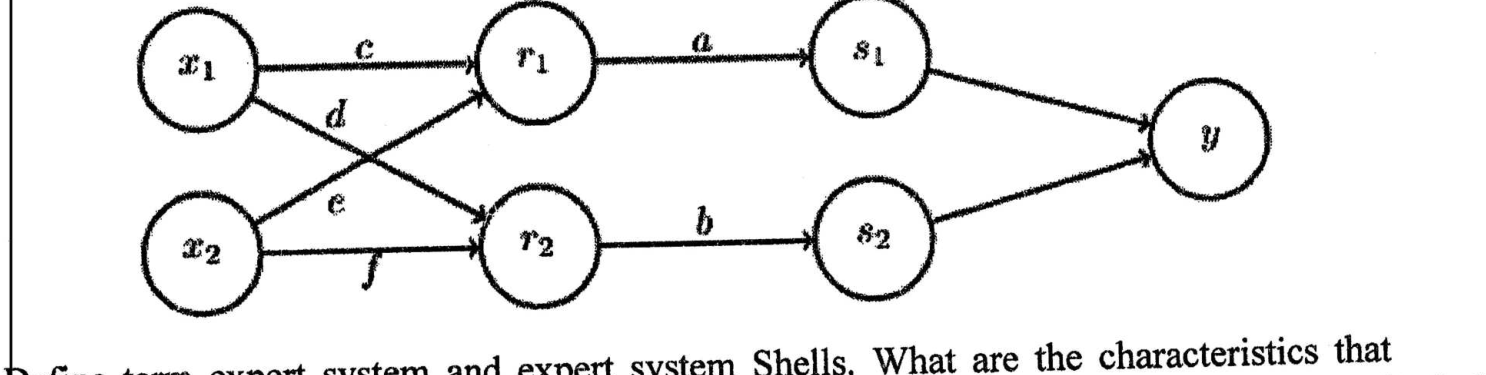
\includegraphics[width=4.6in]{images/ai_82ka_ann.png}\hfill\mbox{}

      \item What is a Hopfield Network? Explain all the steps involved in the Hopfield Network with a suitable example. \hfill [8] (\bo{69 Bh}, \bo{75 Bh})
        \lb What are the features of a Hopfield network? How does a Hopfield network determine active and passive processing units in the network? Clarify with necessary example and illustration. \hfill [8] (\bo{\textit{71 Bh}})
        \lb When do we need a Hopfield Neural Network? Make a comparison between a feed forward network and a Hopfield Network. \hfill [3+5] (80 Ash)
        \lb Design a Hopfield network to store three binary patterns of length 4. Show how to compute the weight matrix and demonstrate the network's ability to recall a pattern from a noisy input. \hfill [6] (\bo{\texttt{82 Bh}})
        \lb Short note: Hopfield Neural Network. \hfill [4] (\bo{80 Ch}) [3] (\texttt{82 Ba})

      \item What is Self-Organizing Map (SOM)? Explain all the steps involved in SOM with a suitable example. \hfill [2+5] (\bo{74 Bh})
        \lb Short note: Self Organizing Map (SOM); Kohonen Network. \hfill [4] (\bo{\texttt{80 Bh}}, \bo{\texttt{79 Bh}}, \bo{75 Bh}, \textit{74 Ma}, \bo{\textit{72 Ash}}) [5] (79 Jth) [3] (\bo{\texttt{81 Bh}})

      \item Compare the following: a) Forward versus backward chaining, b) Hopfield versus Kohonen network, c) Analogy versus Inductive learning. \hfill [3x3] (71 Ma)

      \item Short note: Learning rate; Learning based on statistics; Learning in Neural Network. \hfill [4] (\textit{72 Ma}) [4] (81 Ash)
    \end{enumerate}

  \subsection{Expert System --- architecture, knowledge acquisition, development}
    \begin{enumerate}[topsep=0pt, noitemsep]
      \item Explain different steps of expert system development with an example. \hfill [8] (\bo{69 Bh})
        \lb What is an expert system? Explain the steps of expert system development. \hfill [4+4] (\bo{70 Bh})
        \lb What are the applications of Expert System? Describe the development stages of Expert System briefly. \hfill [2+6] (\bo{73 Bh})
        \lb List the importance of expert system in real life. Draw the block diagram of expert system architecture and explain all blocks. \hfill [2+6] (75 Ba)
        \lb What is expert system? Create a scenario where we require an expert system. List the steps of creating this system. \hfill [2+6] (\bo{79 Ch})
        \lb You need to work as a Knowledge Engineer for a company developing an expert system for Disease Diagnosis. Draw a block diagram and highlight the major steps for development of this expert system. \hfill [6] (\bo{80 Ch})
        \lb You are stuck in a disaster-prone area of Nepal. Give a specific example of how you design an expert system in this scenario with its block diagram. Highlight the key components of the designed system. \hfill [8] (\texttt{82 Ba})

      \item What is an expert system? Explain the general architecture of an expert system. \hfill [8] (69 Po) [2+4] (71 Ma) [1+7] (76 Ba) [8] (\bo{\textit{71 Bh}})
        \lb What are the major characteristics of an expert system? Explain with example. Explain a general approach for developing an expert system with a block diagram. \hfill [2+5] (\texttt{80 Ba})
        \lb What is expert system? Explain how inference is performed in an expert system. \hfill [3+5] (\texttt{81 Ba})
        \lb Draw the block diagram of an expert system and briefly explain each component. List the benefits of using an expert system. \hfill [6+2] (\bo{77 Ch})
        \lb What are expert systems? Explain the architecture of expert system with a suitable block diagram. Highlight the advantages and disadvantages of expert system. \hfill [1+4+3] (\bo{78 Ch})
        \lb Describe Expert System with its architecture. What are its advantages and disadvantages? \hfill [5+2+2] (\bo{\textit{76 Bh}})
        \lb Define Expert System. How does it simulate human reasoning? Explain with example. \hfill [2+5] (\bo{\texttt{82 Bh}})
        \lb Define the term expert system and expert system Shells. What are the characteristics that a problem possesses that are solved by an expert system? Explain with example. \hfill [2+2+3] (82 Ka)

      \item Differentiate between declarative and procedural knowledge. Explain the architecture of an expert system (with practical uses). \hfill [2+6] (70 Ma) [3+6] (72 Ma) [3+5] (73 Ma)
        \lb Differentiate between declarative versus procedural knowledge processing in an expert system. \hfill [6] (\textit{72 Ma})

      \item What is an expert system? Explain its advantages and disadvantages. \hfill [8] (\bo{72 Ash})
        \lb Define Expert System with example. Explain the limitations of Expert System. \hfill [4+3] (\bo{81 Ch})
        \lb Compare expert systems and human experts. Explain each point with suitable practical examples. \hfill [8] (80 Ash)
        \lb Short note: Expert System. \hfill [4] (81 Ash, \bo{\texttt{79 Bh}})

      \item Define knowledge acquisition with example. Explain the architecture of expert system. \hfill [2+6] (\bo{71 Bh})
        \lb How is knowledge acquisition performed in an expert system? Explain one real expert system example with proper architecture. \hfill [2+5] (\bo{74 Bh})
    \end{enumerate}

  \subsection{Natural Language Processing and Machine Vision}
    \begin{enumerate}[topsep=0pt, noitemsep]
      \item What is natural language processing? Explain it. \hfill [6] (\bo{69 Bh})
        \lb What is NLP? Explain the different steps of NLP. \hfill [8] (69 Po) [2+4] (73 Ma) [3+5] (\bo{79 Ch})
        \lb What is Natural Language Processing? Describe the Natural Language Processing steps and its applications. \hfill [2+6] (\bo{72 Ash})
        \lb Justify that NLP is one of the important parts of AI. Explain the steps involved in NLP. \hfill [8] (75 Ba)
        \lb Explain the different steps involved in NLP with a suitable block diagram and examples. \hfill [8] (72 Ma) [7] (\bo{\textit{73 Bh}})
        \lb Define NLU and NLG. List the different steps involved in NLP with suitable examples. \hfill [2+7] (\bo{73 Bh}) [9] (\textit{74 Ma}) [2+6] (\bo{\textit{74 Bh}}, \texttt{82 Ba}) [1+6] (79 Jth)
        \lb What are the problems associated with NLP? List down the different steps involved in NLP with a suitable example. \hfill [2+5] (82 Ka, \bo{81 Ch}) [2+6] (\bo{\textit{77 Ch}})
        \lb What are the problems of natural language understanding? Discuss the steps of NLP. \hfill [3+5] (78 Po)
        \lb Explain the different steps involved in NLP. Why is NLP hard? Explain. \hfill [5+2] (79 Ash)
        \lb What is Natural Language Processing (NLP)? Discuss the different steps in NLP with suitable examples. Also list down the major issues in NLP. \hfill [6+2+2] (\bo{75 Bh})
        \lb Explain the steps of Natural Language Processing. Explain syntactic analysis and draw a parse tree for the following sentence: ``A girl has a name.'' \hfill [5+4] (\bo{\textit{76 Bh}})

      \item Define machine translation in NLP. Explain the challenges of machine translation. \hfill [1+7] (\bo{70 Bh})
        \lb What is NLP? Discuss the different issues related to NLP with example. \hfill [2+6] (70 Ma)
        \lb What is natural language understanding and natural language generation? Briefly list down the steps. Discuss the issues related with NLP. \hfill [2+4+2] (\bo{78 Ch})

      \item What is NLP? Explain the syntactic, semantic and pragmatic analysis of NLP. \hfill [2+2+2+2] (71 Ma)
        \lb Define the following terms: a) Phonetic analysis b) Syntactic analysis c) Semantic analysis d) Pragmatic analysis. \hfill [8] (\bo{\textit{71 Bh}})
        \lb What are the different levels of analysis required in NLP? Justify with one example of each. \hfill [6] (\textit{72 Ma})
        \lb Explain the ambiguity in NLP. Discuss the different steps involved during NLP. \hfill [2+6] (78 Ba)
        \lb Define NLU and NLG. Explain the different ambiguities of Natural Language Processing. \hfill [1+7] (\bo{\textit{72 Ash}})
        \lb How can ambiguity occur at phonetic, syntactic, semantic and pragmatic levels of natural language processing? Give an example. How are syntactic and semantic analysis done during natural language processing? \hfill [3+4] (\bo{\texttt{82 Bh}})

      \item What are the problems associated with NLP? How is syntactic and semantic analysis done during NLP? Explain with example. \hfill [3+5] (\bo{\texttt{80 Bh}}) [2+5] (\texttt{80 Ba})
        \lb List the challenges faced by NLP. Why do you think machine vision is important in AI? Explain with example. \hfill [2+5] (\bo{\texttt{79 Bh}})
        \lb You are hired by a company to work on a product based on the Nepali Language. What are the challenges/issues associated with NLP? List them with appropriate examples and relate these with the Nepali Language. What are your plans to mitigate these challenges while working in the company? \hfill [8] (81 Ash)
        \lb You are hired by a company to develop a Nepali Chatbot System. What are the knowledge bases required to develop the system? List down the different steps involved in the development of this Nepali Language based NLP tool with a suitable block diagram and examples. \hfill [2+6] (\bo{80 Ch})

      \item How does machine vision help in Artificial Intelligence? Explain how the back propagation algorithm helps in machine learning. \hfill [3+5] (71 Ma)
        \lb What is the significant role of machine vision in Artificial Intelligence? Explain how the back propagation algorithm works. \hfill [3+5] (\bo{\textit{72 Ash}})
        \lb What is machine vision? Create a scenario where we require Machine vision. List down the steps of how you solve the above problem. \hfill [2+6] (80 Ash)
        \lb What is Machine Vision? List down the steps involved in Machine Vision by giving a suitable example. \hfill [2+4] (81 Ash) [2+5] (\bo{\texttt{81 Bh}})
        \lb What is machine vision? What are the different steps involved? List down its applications. \hfill [1+5+2] (79 Ash)
        \lb Short note: Machine Vision / Computer Vision / Machine vision applications. \hfill [4] (\bo{69 Bh}, \bo{80 Ch}) [3] (\texttt{80 Ba}, \texttt{82 Ba})

      \item Remaining short notes, by paper: Skolemization and Human Brain verses Neural Network (\bo{69 Bh}); Horn clause (69 Po); Sentence validity (\textit{72 Ma}); Uninformed search (\bo{\textit{77 Ch}}); Breadth first vs depth first search (\bo{75 Bh}). \hfill [various]
    \end{enumerate}

\end{document}
